\documentclass[a4paper]{article}
\usepackage[warn]{mathtext}
\usepackage[utf8]{inputenc}
\usepackage[T2A]{fontenc}

\usepackage[english,russian]{babel}
\usepackage{multicol}
\usepackage{fancyhdr}
\usepackage{graphicx}
\usepackage{microtype}
\usepackage{wrapfig}
\usepackage{amsmath}
\usepackage{floatflt}
\usepackage{geometry} \geometry{verbose,a4paper,tmargin=2cm,bmargin=2cm,lmargin=1.5cm,rmargin=1.5cm}
\usepackage{float}
\usepackage{amssymb}
\usepackage{caption}
\usepackage{epsfig}
\usepackage{newunicodechar}

\usepackage{xcolor}
\usepackage{hyperref}

\usepackage{listings}
\usepackage{color}
 % Цвета для гиперссылок
\definecolor{linkcolor}{HTML}{799B03} % цвет ссылок
\definecolor{urlcolor}{HTML}{799B03} % цвет гиперссылок
 
\hypersetup{pdfstartview=FitH,  linkcolor=linkcolor,urlcolor=urlcolor, colorlinks=true}

\definecolor{dkgreen}{rgb}{0,0.6,0}
\definecolor{gray}{rgb}{0.5,0.5,0.5}
\definecolor{mauve}{rgb}{0.58,0,0.82}

\lstset{
  language=Java,
  aboveskip=3mm,
  belowskip=3mm,
  showstringspaces=false,
  columns=flexible,
  basicstyle={\small\ttfamily},
  numbers=none,
  numberstyle=\tiny\color{gray},
  keywordstyle=\color{blue},
  commentstyle=\color{dkgreen},
  stringstyle=\color{mauve},
  breaklines=false,
  breakatwhitespace=true,
  tabsize=3
}

\begin{document}

\graphicspath{ {pictures/} }

\begin{titlepage}
	\centering
	\vspace{5cm}
    {\scshape\LARGE NetCracker Learning center\par}
	\vspace{5cm}
	{\scshape\Large  Учебное практическое задание № 2 \par}
	\vspace{1cm}
    {\huge\bfseries  Разработать программу с использованием интерфейсов и переопределить методы Java. \par}
	\vspace{1cm}
	\vfill
    \begin{flushright}
        {\large выполнил студент}\par
        \vspace{0.3cm}
        {\LARGE Яромир Водзяновский}
    \end{flushright}
	\vfill
Долгопрудный, 2021
% Bottom of the page
\end{titlepage}

\pagestyle{fancy} 
\fancyhead[L]{Java   $\sim  \hat(\, ^{\circ}  \omega  ^{\circ} \, \hat) \sim$}
\fancyhead[R]{NetCracker}
\fancyfoot[C]{ \noindent\rule{\textwidth}{0.4pt} \thepage }



\newpage 


\textbf{Цель работы: }
Сформировать навыки проектирования и реализации интерфейсов Java, закрепить знания в области разработки классов java и научиться переопределять методы eduals(), hashCode(), toString().

\section{\href{https://github.com/yarvod/NetCracker_LearningCenter/tree/main/Practise_tasks/Practice_task_2/task_1}{Задача №1}}

\textbf{Задание:} Напишите программу, реализующую следующую диаграмму классов: \par

\begin{figure}[H]
    \begin{center}
        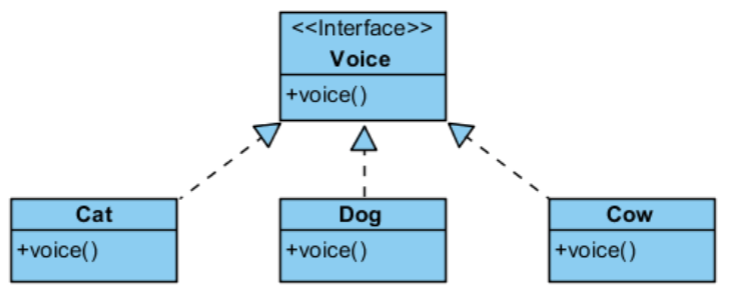
\includegraphics[scale = 0.5]{task1.png}
    \end{center}
\end{figure}

\begin{minipage}{0.5\textwidth}
    \textit{Main.java}
    \begin{lstlisting}
package task_1;

class Cow implements Voice {
    @Override
    public void voice() {
        System.out.println("Myy-myy");
    }
}

class Dog implements Voice {
    @Override
    public void voice() {
        System.out.println("Gav-gav");
    }
}

class Cat implements Voice {
    @Override
    public void voice() {
        System.out.println("Mow-mow");
    }
}
public class Main {
    public static void main(String[] args) {
        Cat cat = new Cat();
        Dog dog = new Dog();
        Cow cow = new Cow();

        System.out.println("Cat: ");
        cat.voice();
        System.out.println("Dog: ");
        dog.voice();
        System.out.println("Cow: ");
        cow.voice();

    }
}   
        \end{lstlisting}
\end{minipage}
\hfill
\begin{minipage}{0.5\textwidth}
        \textit{Voice.java}
        \begin{lstlisting}
package task_1;

public interface Voice {
    void voice();
}
        \end{lstlisting}
\end{minipage}



\newpage

\section{\href{https://github.com/yarvod/NetCracker_LearningCenter/tree/main/Practise_tasks/Practice_task_2/task_2}{Задача №2: Игра в кости}}

\textbf{Задание:} Переработать задачу про игру в кости под использование интерфейсов.
Играют N игроков (компьютер в списке последний). Подкидываются одновременно К кубиков. Выигрывает тот, у кого большая сумма очков. Кто выиграл, тот и кидает первым в следующем кону. Игра идет до 7 выигрышей. Начинаете игру Вы. \par 

\textit{Bones.java}
\begin{lstlisting}
package task_2;

public interface Bones {
    int Play(int K);
    int[] maxArray(int[] Array);
    int[][] Substitute(int[][] PlayerList, int maxScoreIndex);
    void game();
}
\end{lstlisting}

\textit{Main.java}
\begin{lstlisting}
package task_2;

import java.util.Scanner;

class BonesImpl implements Bones {
    @Override
    public int Play(int K) {
        int score = 0;
        for (int j=0; j<K; j++) {
            score += (int) (Math.random() * 6 + 1); 
        }
        return score;  
    }

    @Override
    public int[] maxArray(int[] Array) {
        int index = 0;
        int max = 0;
        int[] maxArray = new int[2];
        for (int i = 0; i<Array.length; i++) {
            if (max <= Array[i]) {
                max = Array[i];
                index = i;
            }
        }
        maxArray[0] = index;
        maxArray[1] = max;
        return maxArray;
    }

    @Override
    public int[][] Substitute(int[][] PlayerList, int maxScoreIndex) {
        int[] save_winner = PlayerList[maxScoreIndex];
        for (int k=0; k<maxScoreIndex; k++) {
            PlayerList[maxScoreIndex - k] = PlayerList[maxScoreIndex - k-1];
        }
        PlayerList[0] = save_winner;
        return PlayerList;
    }

    @Override
    public void game() {

        Scanner in  = new Scanner(System.in);
        int N;
        int K;
        int maxScoreIndex;
        
        System.out.print("Enter number of players: ");
        N = in.nextInt();

        System.out.print("Enter number of cubes: ");
        K = in.nextInt();
        in.close();

        int[] Scores = new int[N];
        int[][] PlayerList = new int[N][2];
        int[] TotalScores = new int[N];
        int WinnerIndex = 0;


        for (int i=0; i<N; i++) {
            PlayerList[i][0] = i;
            PlayerList[i][1] = 0;
        }

        for (int round=0; round<7; round++) {

            System.out.println("Round: " + (round+1));
            for (int player_num=0; player_num<N; player_num++) {
                Scores[player_num] = Play(K);
            }
            maxScoreIndex = maxArray(Scores)[0];

            PlayerList[maxScoreIndex][1] += 1;
            
            for (int k=0; k<N; k++) {
                System.out.println("Player " + PlayerList[k][0] + " has score: " + Scores[k]);
            }

            PlayerList = Substitute(PlayerList, maxScoreIndex);
        }

        System.out.println("Outcomes: ");

        for (int k=0; k<N; k++) {
            System.out.println("Player " + PlayerList[k][0] + " has number of victories: " + PlayerList[k][1]);
        }
        
        for (int i=0; i<N; i++) {
            TotalScores[i] = PlayerList[i][1];
        }

        WinnerIndex = maxArray(TotalScores)[0];
        
        System.out.println("Winner of the Game: Player " + PlayerList[WinnerIndex][0]);

    }
}

public class Main {
    public static void main(String[] args) {
        Bones bones = new BonesImpl();
        bones.game();
    }
}

\end{lstlisting}

\newpage

\section{\href{https://github.com/yarvod/NetCracker_LearningCenter/tree/main/Practise_tasks/Practice_task_2/taks_3}{Задача №3}}

\textbf{Задание: } Напишите программу, реализующую изображенный класс:

\begin{figure}[H]
    \begin{center}
        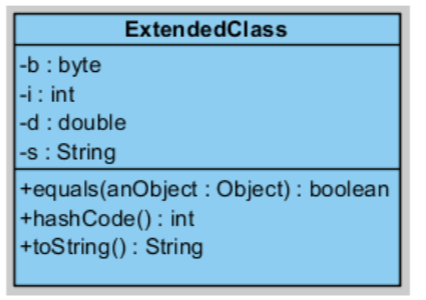
\includegraphics[scale = 0.6]{task3.png}
    \end{center}
\end{figure}

\begin{lstlisting}
package task_3;

import java.util.Objects;

public class ExtendedClass {
    byte b;
    int i;
    double d;
    String s;

    @Override
    public boolean equals(Object anObject) {
        if (anObject == this) {
            return true;
        } else if (anObject == null || anObject.getClass() != this.getClass()) {
            return false;
        }

        ExtendedClass extendedClass = (ExtendedClass) anObject;
        if (this.b == extendedClass.b && this.i  == extendedClass.i && 
        this.d == extendedClass.d && this.s == extendedClass.s) {
            return true;
        } 
        else {
            return false;
        }    
    }

    @Override
    public int hashCode() {
        int result = Objects.hashCode(b);
        result = 31 * result + Objects.hashCode(i);
        result = 31 * result + Objects.hashCode(d);
        result = 31 * result + Objects.hashCode(s);
        return result;
    }

    @Override
    public String toString() {

        return "byte: "+ b + "\n" + "int: " +"i "+ "\n" + "double: " + d + "\n" + "String: " + s ;
    }
}
\end{lstlisting}


\newpage

\section{\href{https://github.com/yarvod/NetCracker_LearningCenter/tree/main/Practise_tasks/Practice_task_2/task_4}{Задача №4, Вариант В}}

\textbf{Задание: }Создайте интерфейс Sleepyс методами sleep(), wakeUp() и ask(). Реализуйте интерфейс в классе SleepyImpl. Метод sleep() устанавливает флаг awake в false, метод wakeUp() в true. Метод ask() печатает в консоль “BOO!”, если флаг установлен в true, и “zzz...” в противном случае. \par


\begin{minipage}{0.5\textwidth}
    \textit{Sleepyc.java}
    \begin{lstlisting}
package task_4;

public interface Sleepyc {
    void sleep();
    void wakeUp();
    void ask();
}
\end{lstlisting}
\textit{Main.java}
\begin{lstlisting}
package task_4;

public class Main {
    public static void main(String[] args) {
        Sleepyc sleepyc = new SleepyImpl();

        sleepyc.sleep();
        sleepyc.ask();

        sleepyc.wakeUp();
        sleepyc.ask();
    }
}
\end{lstlisting}
\end{minipage}
\hfill
\begin{minipage}{0.5\textwidth}
\textit{SleepyImpl.java}
\begin{lstlisting}
package task_4;

public class SleepyImpl implements Sleepyc {
    boolean awake;

    @Override
    public void sleep() {
        this.awake = false;
    }

    @Override
    public void wakeUp() {
        this.awake = true;
    }

    @Override
    public void ask() {
        if (this.awake == true) {
            System.out.println("BOO!");
        } else {
            System.out.println("zzz...");
        }
    }
}
    
\end{lstlisting}
\end{minipage}


\end{document}